\documentclass[12pt]{article}
\usepackage[left=1in, right=1in, top=1in, bottom=1in]{geometry}
\usepackage{graphicx}
\usepackage{url}
\usepackage{cite}
\usepackage{float}
\usepackage{caption}
\usepackage{subcaption}
\usepackage{hyperref}
\hypersetup{
    colorlinks,
    citecolor=black,
    filecolor=black,
    linkcolor=black,
    urlcolor=black
}

\renewcommand{\familydefault}{\sfdefault}


\begin{document}
\begin{titlepage}
    \begin{center}
        \LARGE
        \textbf{ELE 401 - GRADUATION PROJECT I}

        \Large
        \textbf{TERM REPORT}

        \vspace{70pt}

        \textit{
            Hacettepe University \\
            Department of Electrical and Electronics Engineering
        }
    \end{center}

    \vspace{90pt}

    \large

    \textbf{Project Title:} Sensor Fusion in the Cloud \\

    \textbf{Project Group Members:} Ertuğrul Tiyek, Ahmet Yusuf Şirin

    \vspace{30pt}

    \textbf{Project Supervisor:} Asst. Prof. Dr. İsmail Uyanık \\

    \textbf{Submission Date:} 22.01.2023

    \vspace{\fill}

    \begin{center}
        \textit{FALL 2022-2023}
    \end{center}
\end{titlepage}

\clearpage

\tableofcontents
\listoffigures
\listoftables

\clearpage

\begin{abstract}
    One of the most important aim of the modern technology is the sensing the environment. Living beings have sense organs to know the environment. They have brains to make fusion the sensor data and augment the environmental information taken from sense organs. For example, human standing in balance, we can say that they use the data coming from their eyes and ears together.

    People are studying to make this sensing and augmenting artificially, too. They use computers to achieve this. But computers cannot sense the environment directly. They need some devices called sensors. There are all kinds of sensors to measure different environmental quantities. For same quantity, there are different sensors using different technologies, have different precision and accuracy levels. Each sensor has its advantages and disadvantages. Even sensors that are serving a different purpose can help to augment same information other than their main. This is known as "sensor fusion"~\cite{enwiki:1115352853}. Just like humans, robots are use camera and inertial sensors to stand in balance. 

    In our project, sensor fusion handles extracting depth information. Sensor fusion can be implemented using specific algorithms like EKF, CNN etc. according to quantity that will be calculated, number and types of sensors used, accuracy and performance needed. We are planning to develop a sensor fusion algorithm with the help of living organisms. As we mentioned before, living beings perform sensor fusion perfectly. We will be examining the zebra fish and how it processes data of its sense organs to produce depth information. Then we will try to develop similar algorithm or improve our algorithm with data taken from zebra fish. 

    Depth information can be used for many applications like automatic driven vehicles, UAVs, Augmented Reality devices and 3D modeling of areas. Our concept in this project will be autonomous controlled SLAM Robot. Simultaneous localization and mapping (SLAM) is the computational problem of constructing or updating a map of an unknown environment while simultaneously keeping track of an agent's location within it~\cite{enwiki:1120084976}. We use a robot to move the system. 

    Another concept we aim to use is cloud computing. Mobile computing devices may not match the performance requirements in some cases. To achieve more accurate depth information, complex control algorithms or neural networks will be used in our project which needs high computing power. As an alternative to the mobile computing devices, we may use cloud computing.  

    From the point on we are studying on the sensor fusion. In this report we will briefly emphasize the legged robot usage for our final decisions. On the other hand, the concept ot the sensor fusion and the alternative methodologies to implement it correctly to serve the main purpose of sensor fusion, that is reliable odometry data extraction.
\end{abstract}

\section{INTRODUCTION}

One of the most important aim of the modern technology is the sensing the environment. Living beings have sense organs to know the environment. They have brains to make fusion the sensor data and augment the environmental information taken from sense organs. For example, human standing in balance, we can say that they use the data coming from their eyes and ears together.

People are studying to make this sensing and augmenting artificially, too. They use computers to achieve this. But computers cannot sense the environment directly. They need some devices called sensors. There are all kinds of sensors to measure different environmental quantities. For same quantity, there are different sensors using different technologies, have different precision and accuracy levels. Each sensor has its advantages and disadvantages. Even sensors that are serving a different purpose can help to augment same information other than their main. This is known as "sensor fusion"~\cite{enwiki:1115352853}. Just like humans, robots are use camera and inertial sensors to stand in balance.

In our project, sensor fusion handles extracting depth information. Sensor fusion can be implemented using specific algorithms like EKF, CNN etc. according to quantity that will be calculated, number and types of sensors used, accuracy and performance needed. We are planning to develop a sensor fusion algorithm with the help of living organisms. As we mentioned before, living beings perform sensor fusion perfectly. We will be examining the zebra fish and how it processes data of its sense organs to produce depth information. Then we will try to develop similar algorithm or improve our algorithm with data taken from zebra fish.

Depth information can be used for many applications like automatic driven vehicles, UAVs, Augmented Reality devices and 3D modeling of areas. Our concept in this project will be autonomous controlled SLAM Robot. Simultaneous localization and mapping (SLAM) is the computational problem of constructing or updating a map of an unknown environment while simultaneously keeping track of an agent's location within it~\cite{enwiki:1120084976}. We use a robot to move the system.

Another concept we aim to use is cloud computing. Mobile computing devices may not match the performance requirements in some cases. To achieve more accurate depth information, complex control algorithms or neural networks will be used in our project which needs high computing power. As an alternative to the mobile computing devices, we may use cloud computing.

\section{PROJECT DESCRIPTION}

This project aims to construct an unmanned ground vehicle that senses the environment and decides its movements. As mentioned in the "Introduction" section, the sensor fusion and mapping algorithms take a lot of space in this project. In addition to that, there are other parts that need to be implemented like robot controls, data acquisition from sensors and cameras, decision making algorithms etc. 

    \subsubsection*{A. Hardware Architecture of the Project}

    The hardware component choices are explained with consideration of advantages and disadvantages in the section 3.2 Design Constraints. Here we have our main components and specifications of them: 

    \begin{enumerate}
        \item \textbf{Robot – Unitree Go1 Edu} \\
        This robot is a ready-to-go quadruped robot with built-in 5 Sets of Fish-eye Stereo Depth Cameras, Ai Post-processing, 3 Sets of Hypersonic Sensors. There are three Nvidia Jetson Nano, one Raspberry Pi 4, one STM32 Microcontroller devices inside of the Unitree Go1 Edu. These devices located in the robot to perform certain tasks. STM32 Microcontroller drives joint motors of the robot. Raspberry Pi 4 is used for both communicate with user and send commands to STM32. Two of Nvidia Jetson Nano 4GB kits and one Nvidia Jetson Nano 2 GB development kit are used for getting data from camera and sensors, processing raw data to extract dept information of stereo cameras.

        \begin{figure}[H]
            \centering
            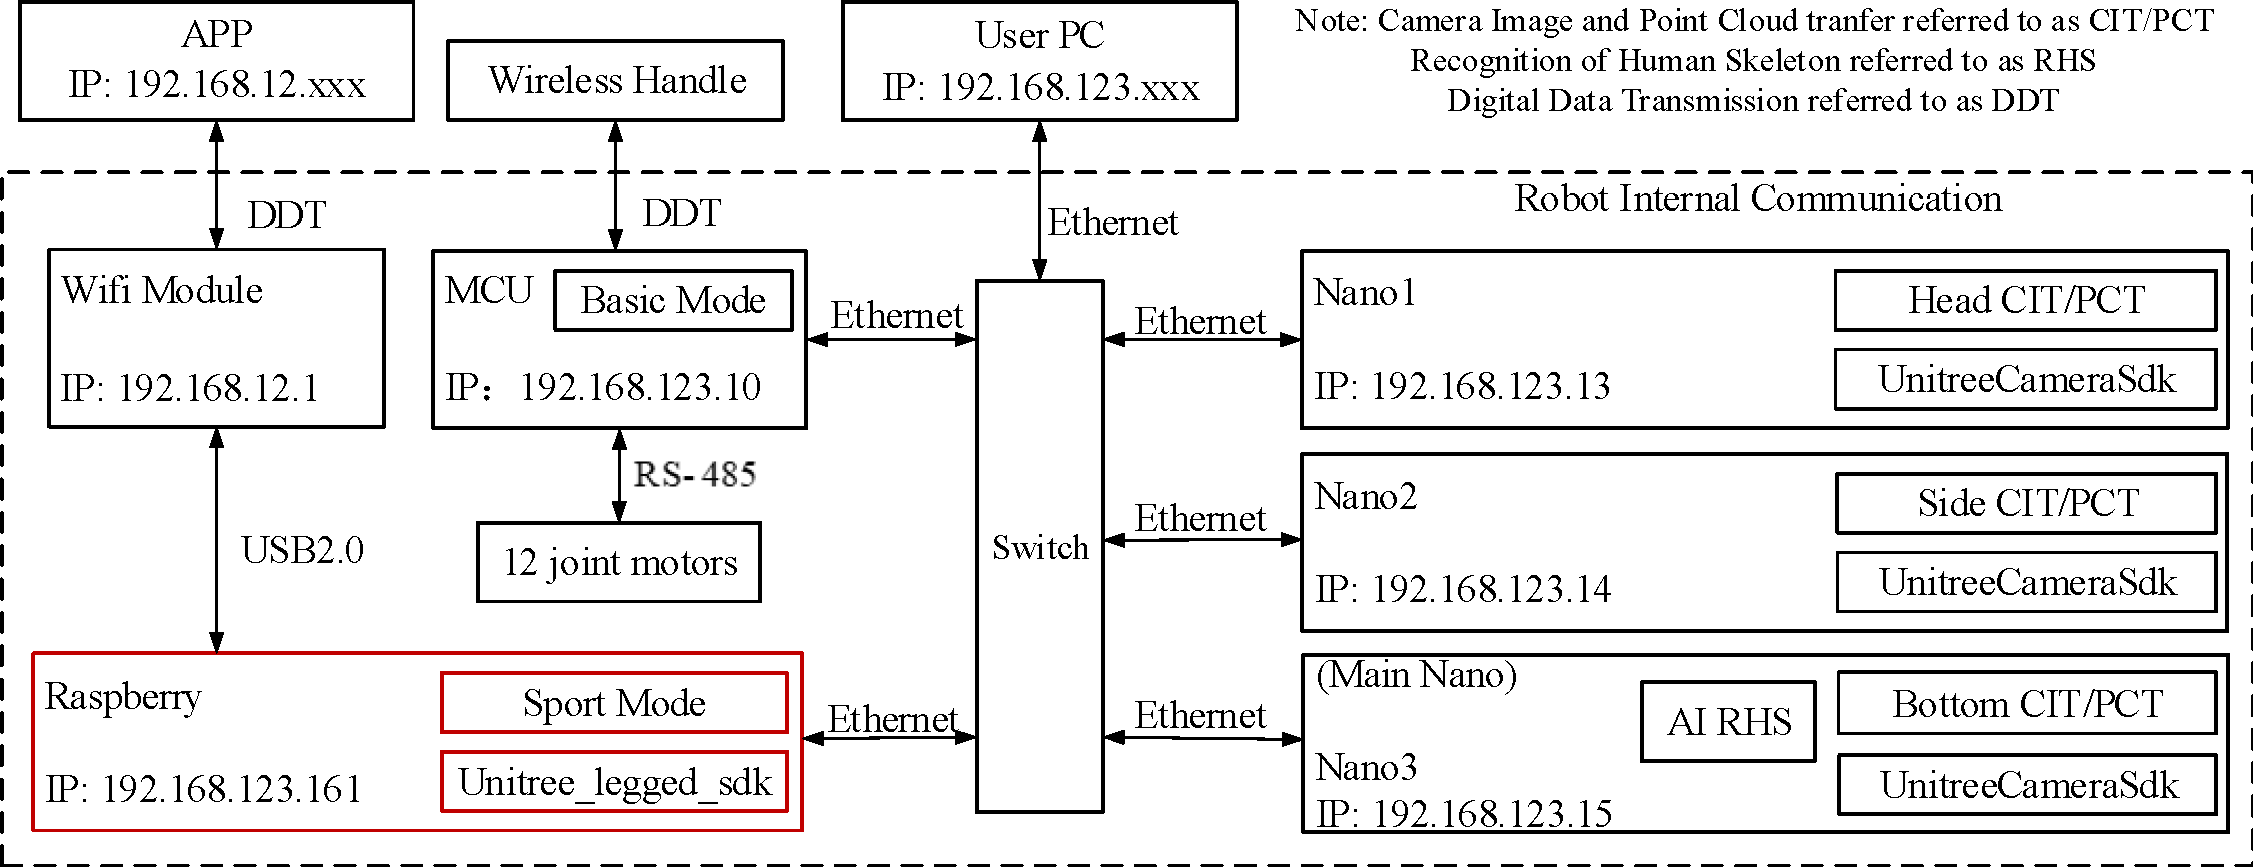
\includegraphics[width=0.9\textwidth]{Go1CommFram_E.png}    
            \caption{Infrastructure of the Unitree Go1 Robot}
        \end{figure}

        The manufacturer provides two Software Development Kits. "unitree\_legged\_sdk” for Controlling the robot, “unitree\_camera\_sdk” for getting camera data and calculating depth information. 

        \item \textbf{Stereo Cameras – Unitree Camera } \\
        There are 5 sets of fish-eye stereo depth cameras located on different important locations of the robot. The known features are:

        \begin{itemize}
            \item Lens Angle $\approx$ 150x170° 
            \item HD (1280x720) , 30fps video streaming 
            \item Raw Frame 
            \item Rectangular Frame 
            \item Depth Frame 
            \item Point Cloud Image 
            \item Provided SDK 
        \end{itemize}
        
        \item \textbf{3D LIDAR – Velodyne 80-VLP-16-A~\cite{VelodyneLiDAR}} \\
        The VLP-16 has a range of 100m, and the sensor's low power consumption (~8W), light weight (830 grams), compact footprint (~Ø103mm x 72mm), and dual return capability make it ideal for UAVs and other mobile applications. 

        Velodyne’s LiDAR Puck supports 16 channels, ~300,000 points/sec, a 360° horizontal field of view and a 30° vertical field of view, with +/- 15° up and down. The Velodyne LiDAR Puck does not have visible rotating parts, making it highly resilient in challenging environments (Rated IP67). 

        Automotive Mapping UAV Security Robotics Automation 

        The module provides up to 0.3 million points/second over 100Mbps ethernet cable and UDP interface. UDP packages contain distances, calibrated reflectivity information, rotation angles, synchronized time stamps (microseconds resolution). 

        \item \textbf{Computation Unit – Nvidia Jetson Nano 4GB} \\
        Unitree Go1 Edu has three Nvidia Jetson Nano Development kits inside it to perform tasks like point cloud, human skeleton tracking etc. We don’t use most of the features robot has, so we decided on using one of the Nvidia Jetson Nano 4GB models in the robot with reducing its 
        workload. 

        Here is some specifications of Nvidia Jetson Nano 4GB~\cite{JatsonNano}: 
        
        \begin{itemize}
            \item GPU		:	128-core Maxwell 
            \item CPU		:	Quad-core ARM A57 @ 1.43 GHz 
            \item Memory	:	4 GB 64-bit LPDDR4 25.6 GB/s 
            \item Storage	:	microSD (not included) 
            \item Camera	:	2x MIPI CSI-2 DPHY lanes 
            \item Connectivity	:	Gigabit Ethernet, M.2 Key E 
            \item Display	:	HDMI and display port 
            \item USB		:	4x USB 3.0, USB 2.0 Micro-B 
            \item Others		:	GPIO, I2C, I2S, SPI, UART 
        \end{itemize}

        As mentioned before, one of the aims of this project is performing heavy computation on cloud. The point of implementing the algorithm on a mobile platform is to keep things simple in the first step. That provides us both simple implementation and ability to make a comparison between mobile computing and cloud computing in terms of performance, accuracy and cost. 

    \end{enumerate}

    \subsubsection*{B. Software Architecture of the Project}

    Laying on the keep it simple stupid (KISS) principle, we separate our project into smaller and independent parts of development.  

    \begin{enumerate}
        \item \textbf{Controlling the Robot Movement and Getting Sensor Data Using Software} \\
        There is a SDK provided by Unitree to control the robot with software called unitree\_legged\_sdk. We used the python programming language with unitree\_legged\_sdk. The details about choice of programming language are explained in the section 3.2 design constraints. 

        Connection between robot and controller computer established via UDP protocol. There are two options that can provide UDP connection. One is the ethernet port of switch that connects all devices in the robot and the other is Wi-Fi access point that connected to the Raspberry Pi 4 in the robot. All devices are using a network mask 255.255.255.0, so it is important to use a static IP on the user computer. 

        \begin{figure}[H]
            \centering
            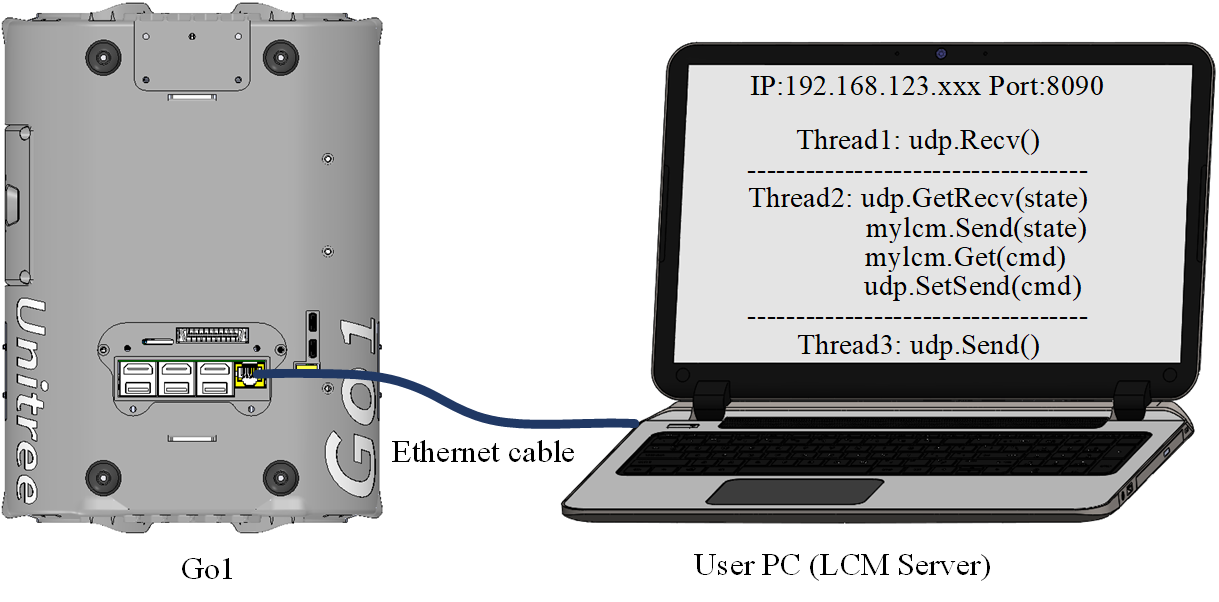
\includegraphics[width=0.8\textwidth]{UserRobotConnection.png}
            \caption{User Robot Connection: Network Mask Settings}
        \end{figure}

        \begin{figure}[H]
            \centering
            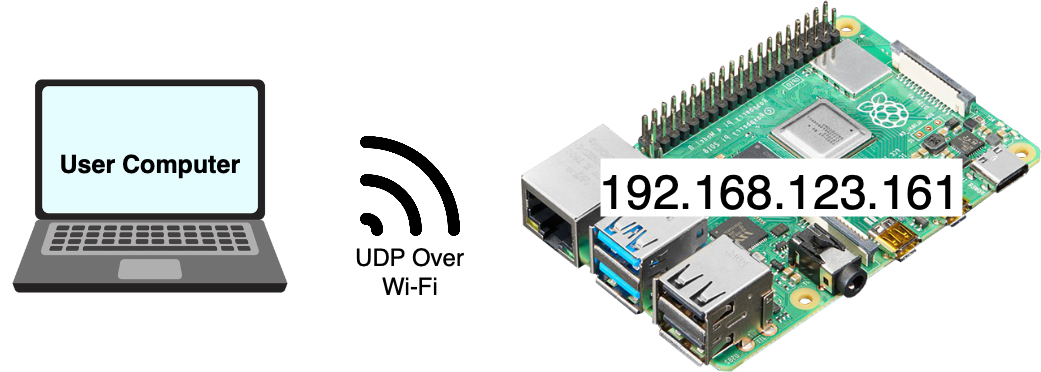
\includegraphics[width=0.8\textwidth]{UserRPiConn.png}
            \caption{User Robot Connection: IP of Raspberry Pi}
        \end{figure}

        Unitree\_legged\_sdk allows both low-level and high-level controls. Low-level control allows user to adjust each joint manually. High-level control provides user to control robot with high-level commands like walk, turn, jump etc. We will be using high-level control for this project. 

        SDK has udp class that provides us an object constructs a UDP connection with Raspberry Pi of Robot. UDP object has functions to receive, send, decode and encode udp packages. 

        Another class included in the SDK is HighState. HighState objects store state information of the robot. It is updated using udp.receive(HighState) function. HighState objects includes IMU measurement information, odometer information, 2D speed information, yaw speed information, position information, body height information etc. 

        To send the commands to the robot, there is a class called CMD in the SDK. CMD object is a command package that tell the robot what to do. CMD package consists of command mode, velocity, yaw speed, target position, required body height variables. Then udp.SetSend(cmd) redyes the cmd object  with encoding it to be sent. Finally the udp object sends the command to the Raspberry Pi using udp.send(). 

        Raspberry Pi 4 also uses unitree\_legged\_sdk to receive commands from and send state information to the user computer. It also communicates with the STM32 Microcontroller which controls all joint motors of the robot. 

        \item \textbf{Getting RGB and Depth Frames from Stereo Cameras (unitree\_camera\_sdk)} \\
        As mentioned before, there are 5 sets of fish-eye stereo depth camera units to both provide an RGB frame and depth frame around the robot.  

        \begin{figure}[H]
            \centering
            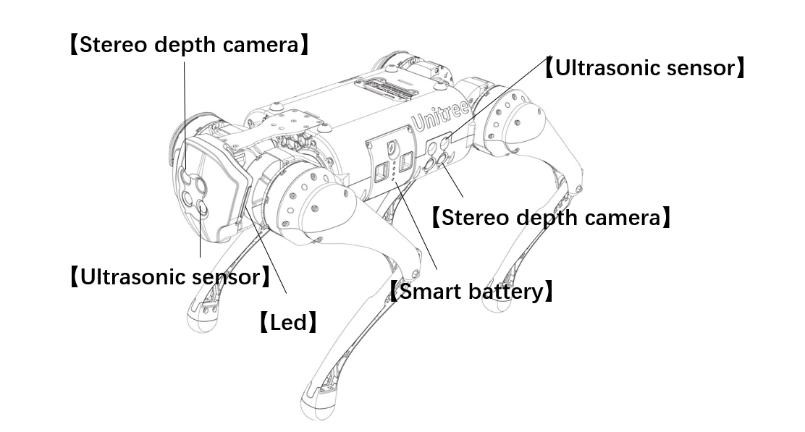
\includegraphics[width=0.8\textwidth]{RobotComponentLocations.jpeg}
            \caption{Legged Robot Sensors and Other Components}
        \end{figure}

        \begin{figure}[H]
            \centering
            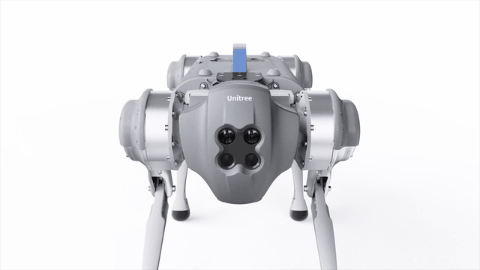
\includegraphics[width=0.8\textwidth]{RobotFront.png}
            \caption{Legged Robot Head Supersensory}
        \end{figure}

        Unitree provides unitree\_camera\_sdk to access camera data of the robot. The SDK allows getting raw frames, rectangular frames, depth frames and point cloud frames. 

        SDK is based on GStreamer framework and works on Nvidia Jetson Nano devices. GStreamer is a library for constructing graphs of media-handling components. Applications can take advantage of advances in codec and filter technology transparently. Developers can add new codecs and filters by writing a simple plugin with a clean, gener~\cite{gstreamer}. GStreamer creates a media pipeline that allows developers to implement their applications simple and modular. 

        unitree\_camera\_sdk creates a pipeline on GStreamer and a virtual video device for each camera connected to the Jetson Nano. Developer can easily read camera information, raw frames, rectangular frames, depth frames and point cloud frames using SDK in their apps. 

        \begin{figure}[H]
            \centering
            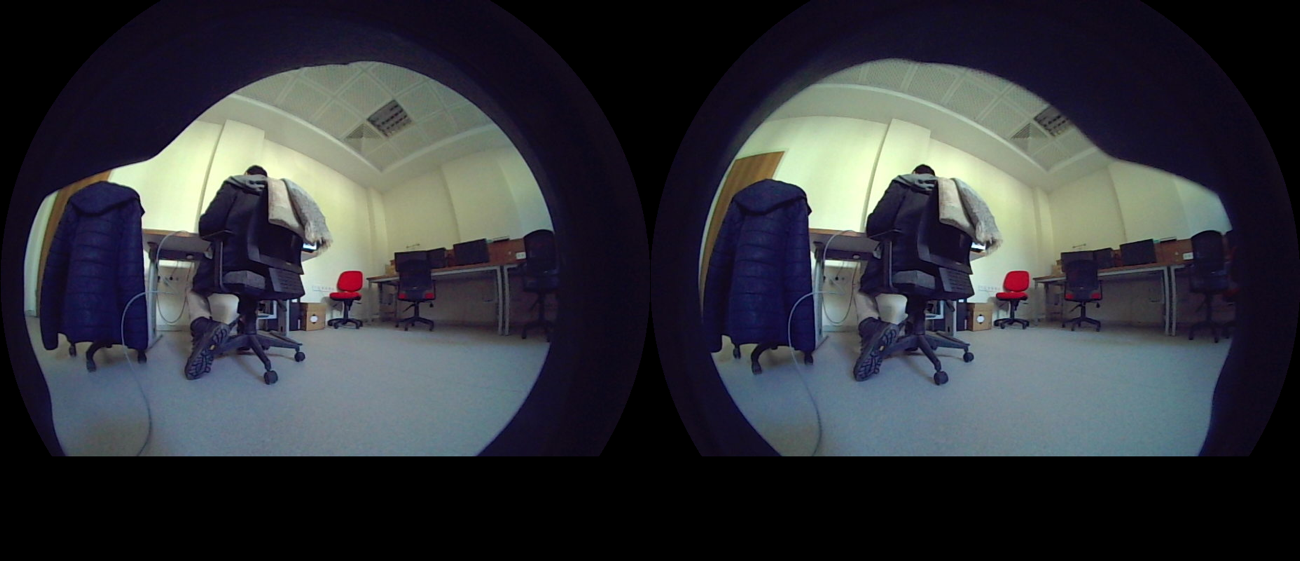
\includegraphics[width=\textwidth]{RawStereo.png}
            \caption{Raw Frame}
        \end{figure}

        \begin{figure}[H]
            \centering
            \begin{subfigure}[b]{0.4\textwidth}
                \centering
                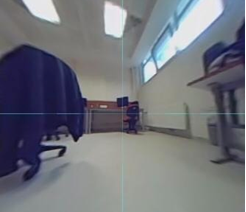
\includegraphics[width=\textwidth]{StereoRectFrame.png}
                \caption{Rectangular Frame}
            \end{subfigure}
            \hfill
            \begin{subfigure}[b]{0.4\textwidth}
                \centering
                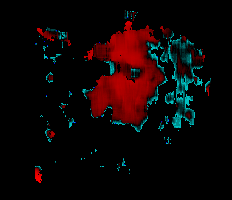
\includegraphics[width=\textwidth]{StereoDeptFrame.png}
                \caption{Depth Frame}
            \end{subfigure}
            \caption{Worked Frames}
        \end{figure}

        Robot has some built in features like human skeleton tracking that uses cameras automatically. There are some services implemented to run these applications automatically while system is starting up. Developer should be whether kill these processes after startup or edit the services not to run processes that uses cameras. 

        Dept information is calculated from stereo camera using stereo vision algorithms. First step is matching each pixel of left frame with corresponding pixel in right frame. This step includes computer vision algorithms like Sum of Squared Differences (SSD) and Sum of Absolute Differences (SAD). 

        \begin{figure}[H]
            \centering
            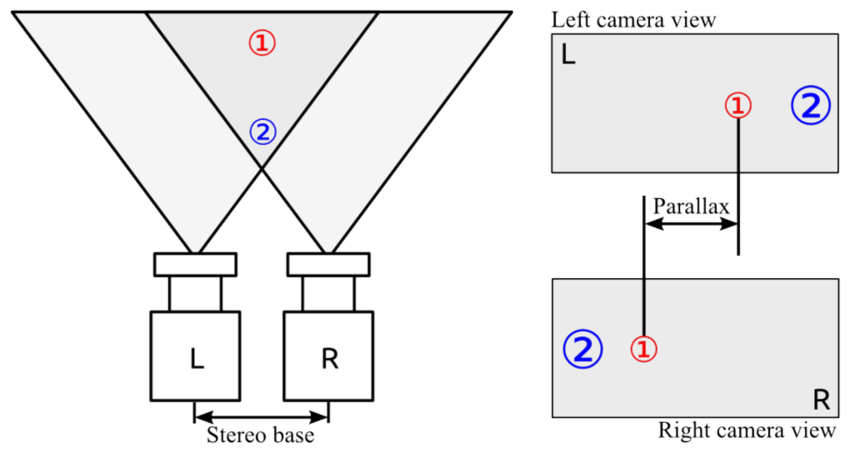
\includegraphics[width=0.8\textwidth]{SSDSAD.png}
            \caption{Sum of Squared Differences (SSD) and Sum of Absolute Differences (SAD)}
        \end{figure}

        After every point matched, distance of every point can be calculated using basic geometric calculations like Thales Theorem. 

        \begin{figure}[H]
            \centering
            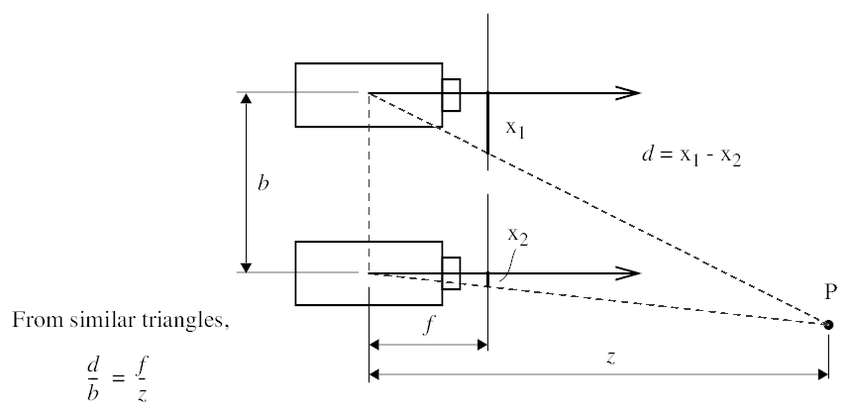
\includegraphics[width=0.8\textwidth]{Thales.png}
            \caption{Thales Theorem}
        \end{figure}

        Stereo cameras provide three dimensional images without using moving parts and high costs. But they have disadvantages as they have advantages. Each camera has lenses to converge and diverge the light coming from different angles and make them fall onto the sensor. That means each camera has a visual angle. Other than that visual angle cannot enter the frame. As we think of the closest points of the baseline of the stereo camera that enters visual angle, it is hard to both match these points in both frames and calculate their distances from camera. Figure shows disparity with respect to distance of the point from baseline of the stereo camera. 

        \begin{figure}[H]
            \centering
            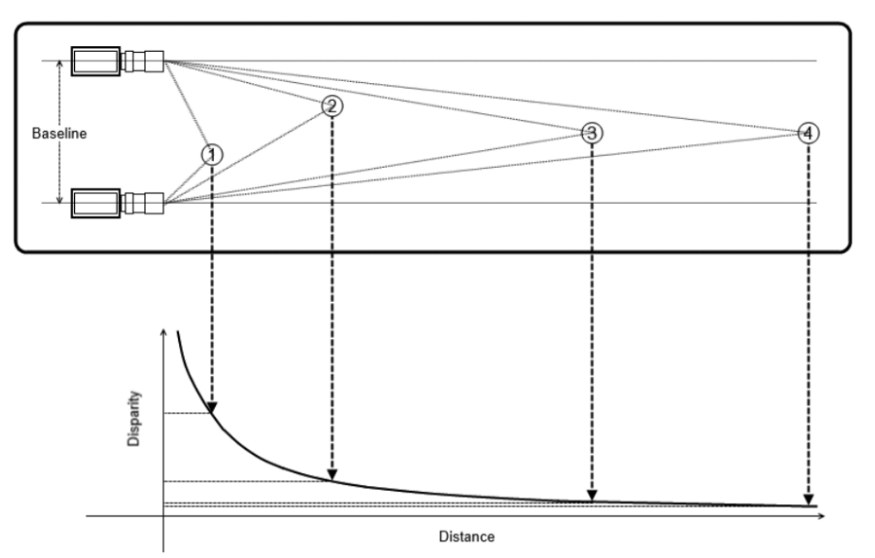
\includegraphics[width=0.6\textwidth]{DisparityOnStereo.png}
            \caption{Disparity with respect to Distance}
        \end{figure}        

        \item \textbf{Developing Sensor Fusion Algorithm for 3D LIDAR and Stereo Cameras}
        \item \textbf{Simultaneously Localization and Mapping (SLAM) }
        \item \textbf{Automating SLAM with Decision Algorithm }
        \item \textbf{Moving Sensor Fusion Algorithm to Cloud}
        \item \textbf{Further Applications Like Swarm Robots with Centralized Cloud System }
    \end{enumerate}

    To accomplish this much work successfully the proof-of-concept parts should be made in a professional manner. In our earlier course work we acquired these experiences by the leading of our course supervisors. Although we will only implement software level designs, the understanding of mathematics and other engineering knowledge cannot be denied. Since we always advice with our supervisor. 

    \begin{table}[H]
        \centering
        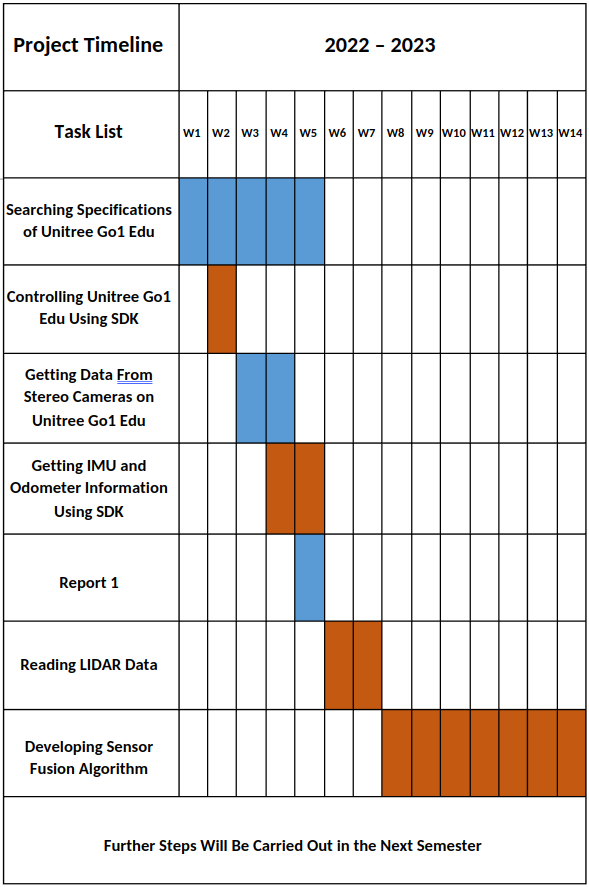
\includegraphics[width=0.65\textwidth]{GanttChart.png}
        \caption{Gantt Chart of Processes}
    \end{table}  

    
\section{ENGINEERING STANDARDS AND DESIGN \\ CONSTRAINTS}

The design constraints should be identified and some discussion on how these apply to the design project and their realization are to be included in this section. You may refer to the list of some realistic design constraints that can be found in the Project Design Constraints document. Other constraints can be identified and discussed, if applicable.  

    \subsection{ENGINEERING STANDARDS}
    
    We use the IEEE standards in our project. From the related pages~\cite{enwiki:1120084976} we found the good to have rules as follows:

    IEEE 829-2008, also known as the 829 Standard for Software and System Test Documentation, was an IEEE standard that specified the form of a set of documents for use in eight defined stages of software testing and system testing, each stage potentially producing its own separate type of document. The standard specified the format of these documents, but did not stipulate whether they must all be produced, nor did it include any criteria regarding adequate content for these documents. These were a matter of judgment outside the purview of the standard~\cite{enwiki:1105776890}. There will be a lot of test cases for the design. Since the system is complex, the test scenarios should be documented with known standard in order to maintenance independently from project contributors.

    A software requirements specification (SRS) is a description of a software system to be developed. It is modeled after business requirements specification (CONOPS). The software requirements specification lays out functional and non-functional requirements, and it may include a set of use cases that describe user interactions that the software must provide to the user for perfect interaction~\cite{enwiki:1117244157}. Since we have such a software system will be developed, it should lay on some standards to make the codes and all implementations reusable and modular.

    A software design description (a.k.a. software design document or SDD; just design document; also Software Design Specification) is a representation of a software design that is to be used for recording design information, addressing various design concerns, and communicating that information to the design’s stakeholders~\cite{enwiki:1105986397}. Similarly, the developed system should have standardized documentation as we said in earlier two standards. The three keywords for a good software design are: modular, reusable, and flexible.

    Of course, as the project progresses, it will be important that we comply with more detailed standards. We will continue to mention these in future reports.


    \subsection{DESIGN CONSTRAINTS}

    From the "Project Design Constraints" document, our constraints are:

    \begin{itemize}
        \item \textbf{Economy:} \\
        For the term project duration we have no spending other then the supervisors did. In case of further production, maintenance, we should spend around 18 dollars without counting the costs of the work put forward. We cannot find this such project on the market. But educational project like ours exist.
          
        \item \textbf{Environment:} \\
        Our robot is battery powered and now on it is only in the development process by different cases. Hence for now we do not have any power consumption calculations (also because we are focused on the software). The radiation we uncovered are on the ISM RF band, legally. And there is no serious pollution of noise, hopefully.

        \item \textbf{Manufacturability:} \\
        Physical implementation will consist of collecting materials and combining them due to use of ready made products. Since, there is no need for high level technologies of manufacturing.

        \item \textbf{Sustainability:} \\
        If we look at the reliability and durability of the design, we can say the legged robot that we use is waterproof but there are a few of external components those are not. Our project is a comprehensive study in which the mathematical foundations of a product that can serve humanity in many areas such as personal use, industrial use and use in disasters are laid and upper engineering problems are solved. In this way, its sustainability is high because it sits on a very comprehensive basis. Also upgrades for scaling purposes are possible to implement since the software we are developing has an abstraction from the hardware. 
        
    \end{itemize}

    and the other constraints for our project specifically due to usage of the some bought products are:

    \begin{itemize}
        \item \textbf{Computing Power}
            \begin{itemize}
                \item \textbf{Internal Nvidia Jetson Nano 4GB:} \\
                Mobile computing devices tend to have less computing power due to their size limits. There are three Nvidia Jetson Nano devices inside of the Unitree Go1 Edu. These devices located in the robot to perform certain tasks. Two of Nvidia Jetson Nano 4GB and one Nvidia Jetson Nano 2 GB development kits are used for getting data from camera and sensors, processing raw data to extract dept information of stereo cameras, human skeleton tracking and so on. 

                We don’t need most of the features of the robot like human tracking in our project, so we can lighten its workload and use one of them as our computing unit. 

                \item \textbf{External Nvidia Jetson:} \\
                In case of having a trouble with using internal Nvidia Jetson device, we can also use an external one. It can be again a Nvidia Jetson Nano with all resources dedicated to our sensor fusion algorithm or a more advanced model like Xavier Nx. This option will rise the cost of the project, so this is an option only if actually needed. 
            
                \item \textbf{Cloud Computing:} \\
                Computing is any goal-oriented activity requiring, benefiting from, or creating computing machinery~\cite{enwiki:1120224488}. There are different computing elements. CPU’s have ability to work high clock frequencies and have large set of sequential instructions. GPU’s are mostly  Mobile computing devices like Nvidia’s Jetson series development kits may not match the performance requirements in some cases. There are GPU servers to provide high parallel computing power.
                
            \end{itemize}

            \vspace{10pt}

            \begin{table}[H]
                \centering
                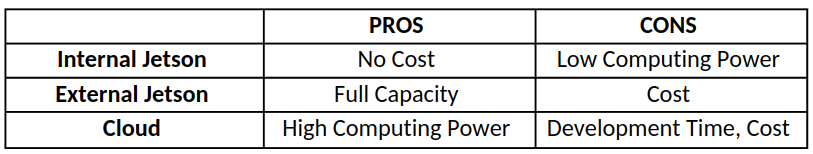
\includegraphics[width=0.8\textwidth]{ComputerComparison.png}
                \caption{Computing Power Comparison}
            \end{table}

            \textbf{Result:} 

            We decided to use Internal Jetson Development kits of the robot for sake of cost reduction. But as mentioned before, one of the aims of this project is moving execution of algorithms that need high computing power to the cloud. So, we will be using both internal Jetson devices and cloud computing. That will be give us an opportunity to compare results in both alternatives. 

        \item \textbf{Depth Sensor \& Stereo Camera}
            \begin{itemize}
                \item \textbf{Internal Unitree Camera – Super Sensory System:} \\
                Lens Angle ~150°×170° 

                \begin{figure}[H]
                    \centering
                    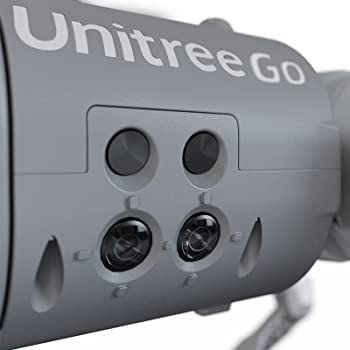
\includegraphics[width=0.5\textwidth]{SuperSensorySystem.png}
                    \caption{Super Sensory System}
                \end{figure}

                \item \textbf{External ZED Stereo Camera:} \\
                
                \begin{figure}[H]
                    \centering
                    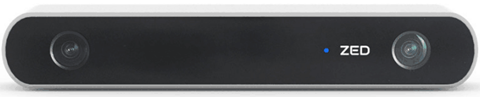
\includegraphics[width=0.5\textwidth]{ZEDCam.png}
                    \caption{ZED Stereo Camera~\cite{ZEDStereoCamera}}
                \end{figure}

                Some specifications of ZED: 

                \begin{itemize}
                    \item High-Resolution and High Frame-rate 3D Video Capture (1080p 30fps) 
                    \item Depth Perception indoors and outdoors at up to 20m 
                    \item 6-DoF Positional Tracking 
                    \item Spatial Mapping 
                    \item 110° Wide Angle Cameras 
                \end{itemize}

                \item \textbf{Xbox 360 Kinect:} \\
                \begin{figure}[H]
                    \centering
                    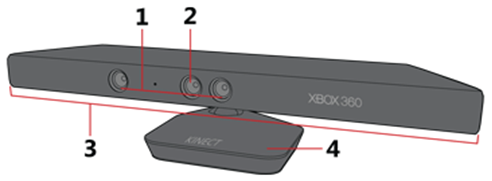
\includegraphics[width=0.5\textwidth]{XBoxKinect.png}
                    \caption{Xbox 360 Kinect~\cite{XboxKinect}}
                \end{figure}

                \begin{enumerate}
                    \item 3D Depth sensor (IR Emitter + IR Camera / Depth Sensor) 
                    \item RGB camera (Color Sensor) 
                    \item Microphone array 
                    \item Tilt motor (for detecting floor and players in the play space) 
                \end{enumerate}

                \item \textbf{Velodyne 80-VLP-16-A 3D LiDAR:} \\
                \begin{figure}[H]
                    \centering
                    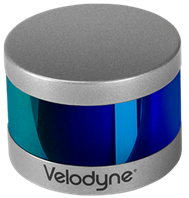
\includegraphics[width=0.3\textwidth]{LiDAR.png}
                    \caption{Velodyne LiDAR}
                \end{figure}

                Some specifications of LiDAR:

                \begin{itemize}
                    \item 100 m Range 
                    \item 360° x 30° Viewing Angle 
                    \item 0.3 Million Points/Second 
                    \item 100Mbps Ethernet \& UDP Interface 
                    \item Rated IP67 
                \end{itemize}
            \end{itemize}
        
        \vspace{10pt}

        \begin{table}[H]
            \centering
            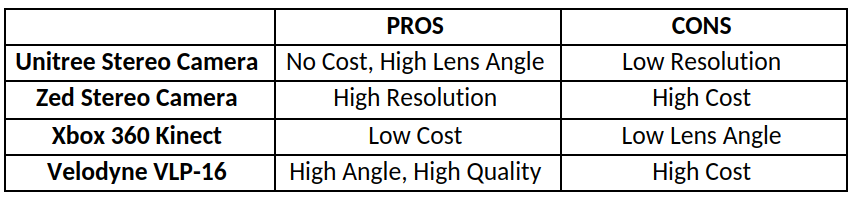
\includegraphics[width=0.8\textwidth]{SensorProsCons.png}
            \caption{Sensor Comparison}
        \end{table}

        \textbf{Result:} 

        As we consider the trade-offs that are given at table-x, we decided to move on with Unitree Stereo Cameras and Velodyne VLP-16 3D Lidar. 

        \item \textbf{Programming Languages} \\
        There are different tools we need to use to control the robot, access its sensor measurements and camera data etc. The robot manufacturer provides SDKs to access and control the robot. These SDKs are implemented using C++ programming language. 

        There is an SDK provided by Unitree to control robots with software. The SDK is implemented in C/C++ languages, but it supports programming in C, C++ and Python languages. So, at some point, we had to use those languages. 

        Besides these, ROS technology has a lot of programming languages provided. Since, we have no restriction from this side, hopefully. 

        \vspace{10pt}

        \textbf{Result:} 

        As we consider the performance and easy usage, we are planning to use Python only for algorithm development. After that we will be implement same algorithms in C++ to improve performance. SDK handles most of the ROS work, but we use ROS commands if it needed. 
        
    \end{itemize}


\section{SUSTAINABLE DEVELOPMENT GOALS}

Our project is a comprehensive study in which the mathematical foundations of a product that can serve humanity in many areas such as personal use, industrial use and use in disasters are laid and upper engineering problems are solved. In this way, its sustainability is high because it sits on a very comprehensive basis. If we look at our project in the context of global goals, it is a good example of Goal 9: Industry, Innovation, and Infrastructure. In addition, our design successfully complies with Goal 12: Responsible consumption and production, as abstractions are kept neatly. For example, scaling in design using the same software infrastructure is quite possible and simple.


\section{BACKGROUND}

For this project the need of strong background is irrefutable. Since there is software oriented design for our case, the reasearchs are more leading. Background comes from the earlier courses in our department, additional research, professional life, and even daily life. Also tricky parts are coming from experiences of our supervisors (know-hows, etc.).

    \subsection{BACKGROUND ACQUIRED IN EARLIER COURSE WORK}

    The sensor fusion operation require a lot mathematical theory and its practical implementations. At this point, the importance of our Calculus (MAT123/124) and Engineering Mathematics (MAT235/236), Signals and Systems (ELE301), Control Systems (ELE354), and Digital Signal Processing (ELE407) courses takes place. 

    But they are not enough to come up with a practical project. To design the system of this large computing environment and the network we should lay on the Computers and Programming (ELE107), Computer Programming (ELE118/120), Data Structures (ELE411), and Data Communication (ELE412) courses. For the sensor fusion operation we also use the knowledge from the Image Processing (ELE492) course for filtering bases and the hands-on programming purposes.

    \subsection{BACKGROUND ACQUIRED THROUGH ADDITIONAL\\ RESEARCH}

    Although our courses that we took in our department are pretty important for the theoretical base and introductory for the implementation, the know-hows of the programming languages, computer architectures, design patterns, and the protocols that we use are beyond from the course curriculums. To get those knowledge, we made a lot of research about those. Besides this, specifically the programming language practices are coming from our part-time jobs, internships, extracurricular studies, and further studies, and coding practices which coming from our supervisors suggestions.

    To be more specific, the CPP and the Python programming languages are not taught but we should already know those to go further in our design. Another example is ROS (robot operating system) concept that is special for our purposes has nothing to do with our courses. Sensor fusion is also a specific research area of the digital signal processing, control systems, mathematics, and Computer Vision~\cite{enwiki:1120271364} for ur case, obviously. Hence, we also made lots of preliminary study in this topic, other than courses.
    

\section{METHODS}

The definition of our project is explained in detail in the first interim report. In the light of the definition, we try to make the decisions and the design parameters clear. To sake of easiness we draw some paths going same destination and arguing to reach the optimal path on the alternatives. Those alternatives are listed and described below. Then we will clearly elucidate our method now.

Since the project includes plenty of areas to work those are distinct, we divide them into subtopics. Those are:

\begin{enumerate}
    \item Sensor Choosing Methods
    \item Sensor Fusion Methods
    \item Sensor Data Enhancement Methods
    \item Fusion Data Enhancement Methods
\end{enumerate}

\subsection{Sensor Choosing Methods}

Our aim in this project is to achieve high reliability by using (fusing) all the sensors we have together. However, when we want to do all these together, we foresee that the project will reach very different dimensions. Therefore, while continuing the project, we decided to select a number of sensors in order to focus on algorithm development.

We set ourselves criteria when choosing sensors. Easy to use sensors is one of our main priorities due to our job description. In addition, considering the algorithmic complexity, working with sensors with linear system response is also an important criterion. In addition, the frequency of receiving data from the sensor is of great importance. Because if the sensor data we will fuse does not come at the same frequency, we will need to add operations to our algorithm to make the sensor frequencies equal by upsampling and downsampling.

We basically divided the sensors we have into two groups as those producing RGBD data or those producing Depth Point Cloud data.

\subsubsection{Method 1: Internal Sensor Using}
The internal sensors of the legged robot include five pairs of stereo cameras that produce RGBD data, and ultrasonic sensors that produce Depth Point Cloud data when viewed cumulatively, SuperSensorySystem. In addition to these, each foot has pressure sensors and an internal IMU.

\subsubsection{Method 2: External Sensor Using}
Our external sensors are ZED Stereo camera which produces RGBD data, Velodyne 3D LiDAR which produces Depth Point Cloud data and Xbox 360 Kinect having 3D depth sensor, RGB camera, microphone array, and also tilt motor. In the future, it is also possible to add sensors such as IMU and GPS to support odometry information.

\subsubsection{Method 3: Mixed Sensor Using}
We can also use our sensors mixed. However, complexity will increase in this method and the workload to be done before the sensor fusion algorithm will become more.


\begin{itemize}
    \item \textbf{Internal Unitree Camera – Super Sensory System:} \\
          Lens Angle ~150°×170°

          \begin{figure}[H]
              \centering
              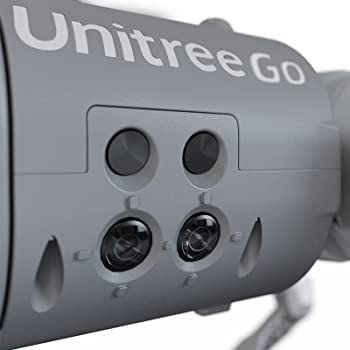
\includegraphics[width=0.5\textwidth]{SuperSensorySystem.png}
              \caption{Super Sensory System}
          \end{figure}

    \item \textbf{External ZED Stereo Camera:} \\

          \begin{figure}[H]
              \centering
              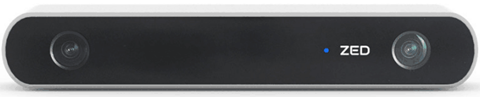
\includegraphics[width=0.5\textwidth]{ZEDCam.png}
              \caption{ZED Stereo Camera~\cite{ZEDStereoCamera}}
          \end{figure}

          Some specifications of ZED:

          \begin{itemize}
              \item High-Resolution and High Frame-rate 3D Video Capture (1080p 30fps)
              \item Depth Perception indoors and outdoors at up to 20m
              \item 6-DoF Positional Tracking
              \item Spatial Mapping
              \item 110° Wide Angle Cameras
          \end{itemize}

    \item \textbf{Xbox 360 Kinect:} \\
          \begin{figure}[H]
              \centering
              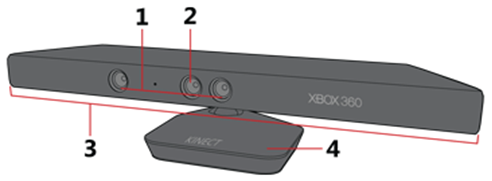
\includegraphics[width=0.5\textwidth]{XBoxKinect.png}
              \caption{Xbox 360 Kinect~\cite{XboxKinect}}
          \end{figure}

          \begin{enumerate}
              \item 3D Depth sensor (IR Emitter + IR Camera / Depth Sensor)
              \item RGB camera (Color Sensor)
              \item Microphone array
              \item Tilt motor (for detecting floor and players in the play space)
          \end{enumerate}

    \item \textbf{Velodyne 80-VLP-16-A 3D LiDAR:} \\
          \begin{figure}[H]
              \centering
              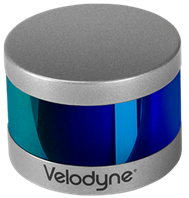
\includegraphics[width=0.3\textwidth]{LiDAR.png}
              \caption{Velodyne LiDAR}
          \end{figure}

          Some specifications of LiDAR:

          \begin{itemize}
              \item 100 m Range
              \item 360° x 30° Viewing Angle
              \item 0.3 Million Points/Second
              \item 100Mbps Ethernet \& UDP Interface
              \item Rated IP67
          \end{itemize}
\end{itemize}

We have taken all these into consideration while doing the preliminary design, and together with the evaluations under the following headings, we have determined a starting point for ourselves. You can find the details under the Preliminary design heading.

% Stereo Camera Decision Method
% LiDAR Decision Method
% Internal IMU usage on legged robot
% Documentation about sensors in marketplace and we owned (engineering decisions on costs)


\subsection{Sensor Fusion Methods}

\subsubsection{Method 1: Complementary Filter}
We wanted to set out using known methods for sensor fusion. In this way, we aimed to improve the performance we want to achieve with methods that we understand fundamentally, instead of using the resources in the literature directly. In fact, we started out by examining the usages of Kalman filter and extended Kalman filter, which are quite commonly used for state estimations made from aircraft IMU sensors, in this field. We predicted that if you continue on your way by choosing the most primitive complementary filter among them, we will be able to understand more clearly that we are moving away from the target in every development we make.

\begin{figure}[H]
    \centering
    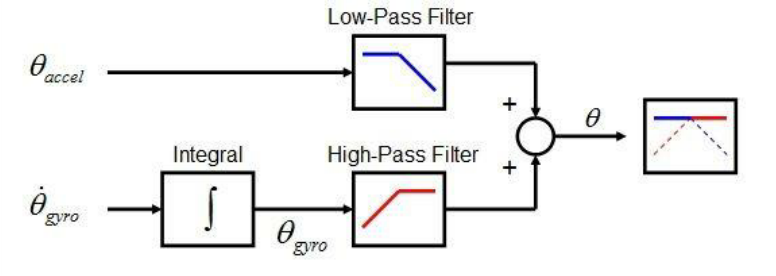
\includegraphics[width=0.7\textwidth]{CF.png}
    \caption{Complementary Filter Example for Aircraft Attitude}
\end{figure}

\subsubsection{Method 2: Kalman Filter}
Using the Kalman filter is also a method between using the extended Kalman filter and using a complementary filter. Since we want to use it with some methods that will enhance compelemntery filtery, we have already produced our own gain function. However, we also considered the Kalman filter as a method.

\begin{figure}[H]
    \centering
    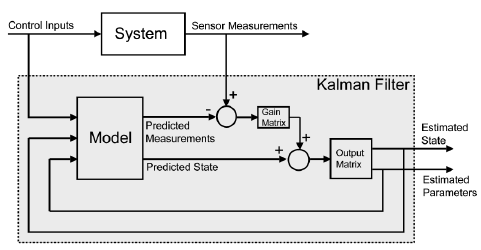
\includegraphics[width=0.7\textwidth]{KF.png}
    \caption{Kalman Filter Example for Aircraft Attitude}
\end{figure}

\subsubsection{Method 3: Extended Kalman Filter Method}
In addition to previous methods, we also evaluated the opinion that preliminary design can speed up the process by directly using the most advanced extenden Kalman filter. However, unlike in the aircraft scenario, we could not find an example use for depth data to be suitable for our scenario~\cite{9307398}.

\begin{figure}[H]
    \centering
    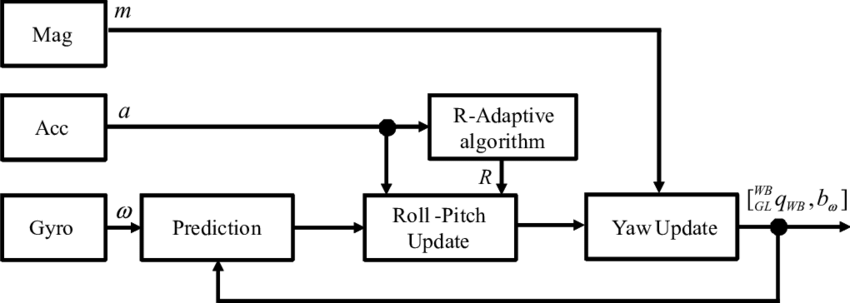
\includegraphics[width=0.7\textwidth]{EKF.png}
    \caption{Extended Kalman Filter Example for Aircraft Attitude}
\end{figure}

A comparison in which the models in which the state estimator methods are effective and the noise characteristics are given together is given in the X table, cost function comparisons for further analysis~\cite{The_cost_function_of_the_data_fusion_process_and_i}.

\begin{table}[H]
    \centering
    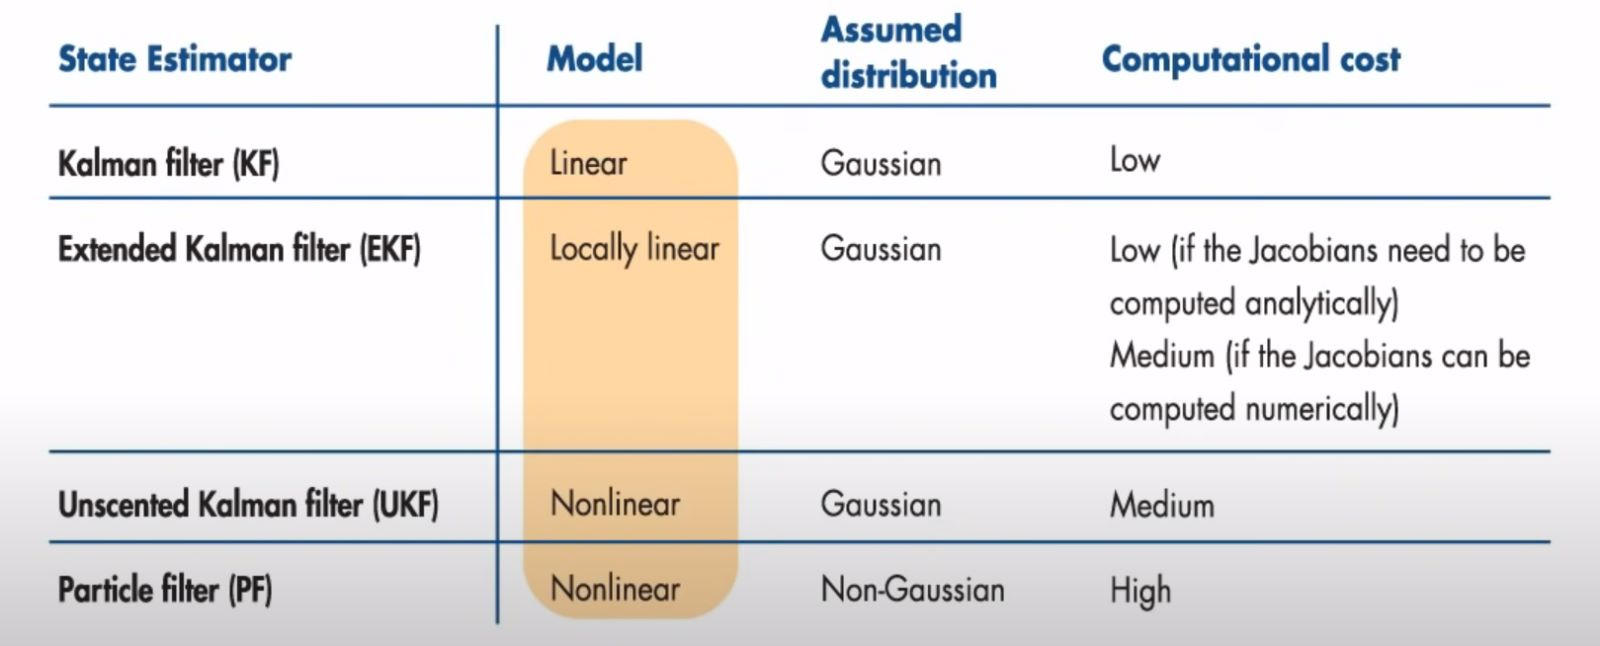
\includegraphics[width=0.8\textwidth]{CostComparison.jpeg}
    \caption{Cost Function Comparison}
\end{table}


\subsection{Sensor Data Enhancement Methods}

We compare the following methods for data enhancement to following data fusion.

\subsubsection{Method 1: Only Data Rate and Range Matching}
Since the data we want to obtain is odometry, we evaluated creating parametric inputs in the methods we used while continuing the project. Because we sould think about Sensor Data Rate - State Estimation Relation. In this way, we aimed to analyze whether we could establish a relationship between the quality of the raw data and the esimated odometry data. After some tests we will briefly report our results about early sensor data enhancement for sensor fusion.

\subsubsection{Metod 2: Papoulis-Gerchberg Algorithm for Depth Point Cloud}
We are searching about Papoulis-Gerchberg algorithm effects on LiDAR and Stereo depth map results to enhance the data resolution before data fusion. An image super-resolution method, the Papoulis–Gerchberg (P–G) algorithm, on range data represented in the form of a greyscale image. However, the low convergence rate of the original P–G algorithm impedes its use for online applications~\cite{ozbay2015high, kuzucu2018enhancing}. By referencing this method we also proposed as an enhancement method.~\cite{6280128}


\section{PRELIMINARY DESIGN}

ZED stereo camera and Velodyne 3D LiDAR were chosen for the preliminary design, which are sensors that are well-documented, have a large community, and are easier to use and access resources than the internal sensors of the legged robot. This sensor will also minimize the complexity of the algorithm to be used in sensor fusion, as they offer a wide resolution and data rate band.

As the sensor fusion algorithm, it was ordered from simple to complex or from low to high performance, and it was decided to make a start with a complementary filter. Again, it was decided to use methods such as edge preservation~\cite{9307398} as an aid to the main algorithm in order to increase the sensor fusion performance.

We choose the complementary filter for fusing the depth information of two sensors. Each sensor has its own properties, advantages and disadvantages. According to these characteristics of sensors we tune our sensor fusion algorithm. But like all control systems, we first regulate our input signals to work with.

Thing we have to match in these two sensors data is viewing angle. Stereo vision camera has a viewing angle upto 110°. We simply reduced the viewing angle of the 3D lidar to match the stereo vision cameras viewing angle. But further steps we are planning to use also 360° lidar information to enhance environmental data while performing SLAM.

Raw data provided by lidar and stereo vision cameras in different formats. Stereo vision camera extracts depth frames as well as RGBD (Red Green Blue Depth) in cartesian form. 3D lidar extracts data in point cloud form which is basically in spherical form. In the other hand the resolution of stereo vision data is available in 2208x1242 at 15 fps, 1920x1080 at 30fps, 1280x720 at 60 fps, 672x376 at 100 fps. The 3D lidar works completely different and samples much less data. In order to match the sampled data from two sensors, we decided upsampling the lidar data and converting it to cartesian form. We use dynamic Papoulis–Gerchberg algorithm to augment the lidar data and then linearly interpolate this information while converting point cloud data to depth frame.

Iterative Papoulis–Gerchberg algorithm is the method used to recover the lost samples of the signal. It is mostly used for super resolution images in image processing. In a single frame manner, iterative Papoulis–Gerchberg algorithm will be enough to increase data in a single point cloud of a lidar. But our aim is continuously matching the frames, we will use the dynamic Papoulis–Gerchberg algorithm. This algorithm make use of stillness of background and continuity of movement to reduce computational effort in Papoulis–Gerchberg.

There is also difference between sample rates of two sensors. Stereo camera samples frames in range of 15 to 100 frames per second. Lidar samples point clouds by rotating its lidar continuously. Each rotation provides one whole 360° sample (30° vertical). Lidar works in range 300 rpms to 600 rpms. That provides us 5-to-10 point clouds per second. We aim to up-sample the  number of point cloud per second by again linear interpolation.

There is one more problem with the lidar. Ability of lidar is not limited by the only rotation but also sample rate of sensor. Increasing rotation speed reduces the quality of the point clouds. One part of the project is experiencing the different data rates and calculating the processing effort, transmission capabilities and response times. So we will optimize resolution and data rates in the content of this project.

\subsection*{Sensor Fusion Algorithm}

We matched the formats of the input signals to keep the sensor fusion simple. There are two depth images as input signals to get more accurate depth image.

As a preliminary design, we are planning to calculate the depth image in per pixel fashion. As mentioned before, the complementary filter is formulated as:

\begin{equation}
    \hat{x} = \hat{x}_1 \alpha + \hat{x}_2 (1 - \alpha)
\end{equation}

We will generate $\alpha$ generation function to calculate $\alpha$ for each pixel and condition. Input sources are not functioning perfect in every conditions. There are some internal and external variables that effects the accuracy of measurement. Let’s observe these variables:


\subsubsection*{Variables That Effect Lidar:}

\begin{itemize}
    \item Beam Angle:

          3D lidar scans the environment in a three-dimensional manner. Velodyne VLP-16 scans 360° horizontally and 30° vertically. In different beam angles, Lidar accuracy depends. There is an article that contains more information about beam angle effect.

          \begin{figure}[H]
              \centering
              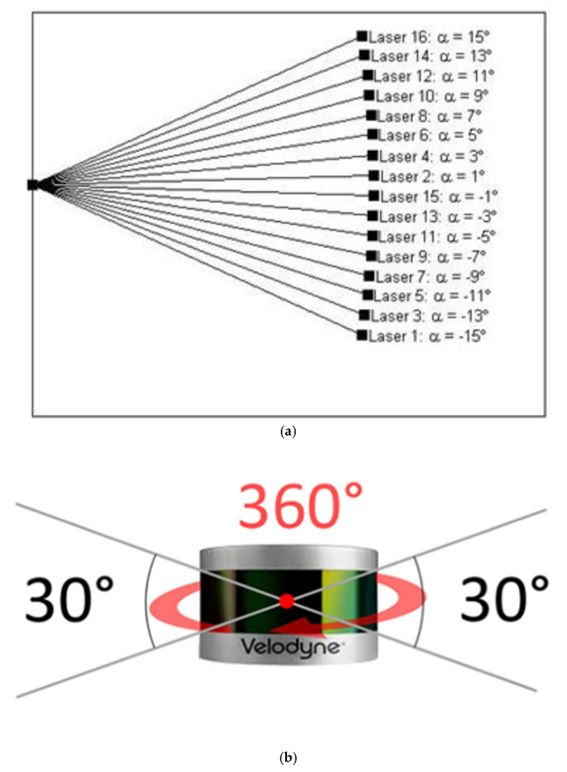
\includegraphics[width=0.5\textwidth]{LidarAngles.jpeg}
              \caption{Velodyne LiDAR Beam Angles~\cite{VelodynePerformance}}
          \end{figure}

    \item Rotation Speed:

          Sample rate of the lidar decreases as rotation speed of the lidar increases. It effects the quality of the depth image. But increasing the rotation speed provides us approximation to real time application.

    \item Distance:

          3D lidars can work in a range that is specified in datasheet. Out of this range, lidar cannot work properly. As we think of the working principle of the lidar, the processing time is not enough to measure too close points. The Velodyne VLP-16 model has a working range between 1m to 100m.

    \item Rough and Uneven Views:

          The Lidar is using wavelengths very close to visible light to observe visible objects. In some environments like forests, rough areas, rainy and foggy weathers there are lots of indentations like branches, twigs and leaves or water drops. Each of this bits and pieces prevents the infrared laser lights coming from lidar and creates canopies. Instead of a clean point cloud, lidar gets a noisy one.

          We can measure the effect of the bits and pieces in the environment to accuracy of lidar measurement by calculating the gradient of depth frame around target pixel.

          \begin{figure}[H]
              \centering
              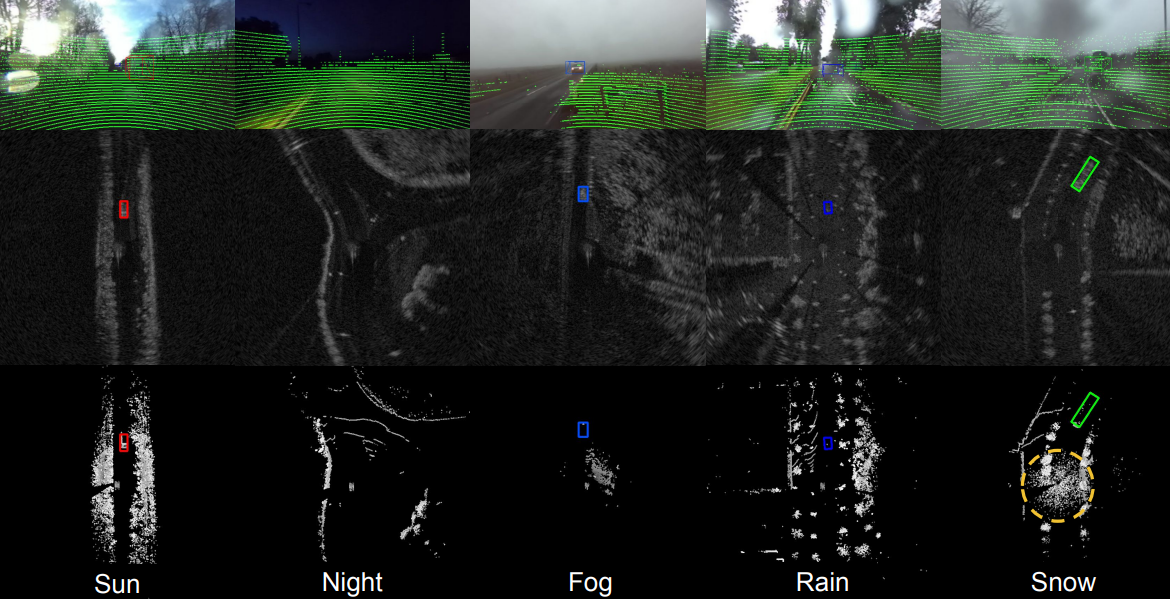
\includegraphics[width=0.9\textwidth]{LidarViews.png}
              \caption{Gradient of Depth Image Around Target Pixel Gives Roughness of the Environment~\cite{https://doi.org/10.48550/arxiv.2010.09076}}
          \end{figure}
\end{itemize}


\subsubsection*{Variables That Effect Stereo Vision Camera:}

\begin{itemize}
    \item Distance:

          According to viewing angles and algorithm used to extract depth information from stereo image, there is an uncertainty appears. And this uncertainty increases as distance of the pixel increases. Uncertainty reduces the confidence of the input as it increased.

          \begin{figure}[H]
              \centering
              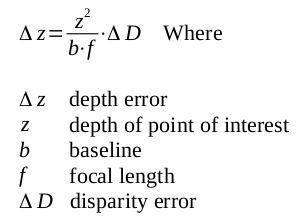
\includegraphics[width=0.4\textwidth]{CamDistance.png}
              \caption{Stereo Camera Depth Error Calculation~\cite{DisparityCalculator, gallup2008variable}}
          \end{figure}

    \item Brightness:

          The brightness of the environment is important for stereo vision depth estimation. As considering the working principles of the stereo vision depth estimation, there are two frames taken from different angles. First step is matching each pixel of left frame with corresponding pixel in right frame. This step includes computer vision algorithms like Sum of Squared Differences (SSD) and Sum of Absolute Differences (SAD). To perform matching properly, the frames should have well distributed histograms and good contrast values. If there is the brightness of frames are too high or too low, the algorithms cannot match the corresponding pixels.

          We can calculate the effect of brightness by observing the histogram of the RGB frames.
    \item Straight and no-Contrast Views:

          Like the brightness, the content of the frame is also important. If the frame includes low contrast, straight or similar patterns, the matching algorithms won’t work properly. For example, If the frame includes a flat white wall, the algorithm can not distinguish pixels in different frames. Likewise, if the frame has a periodic pattern like damas pattern, the algorithm also not work well.

          In this case we can calculate the effect of straightness by calculating gradient around target pixel in RGB frames.
\end{itemize}

According to these parameters, we will derive confidence generator functions that will calculate a confidence value for each input. By normalizing one of the confidence values will give us $\alpha$ value.

\begin{equation}
    \alpha = \frac{C_{LIDAR}}{C_{LIDAR} + C_{STEREO}}
\end{equation}

\begin{figure}[H]
    \centering
    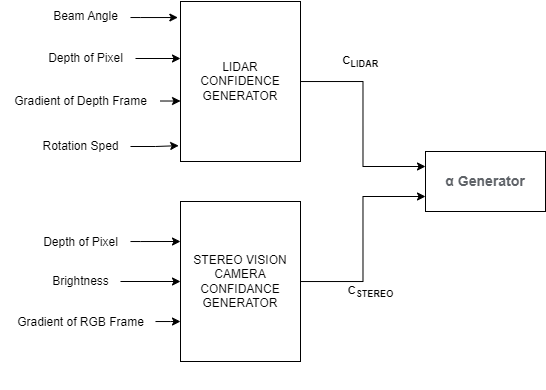
\includegraphics[width=0.9\textwidth]{AlphaFunction.jpeg}
    \caption{Alpha Function for Complementary Filter Enhancement}
\end{figure}

After extracting $\alpha$ value for each pixel of depth frame, we can simply apply complementary filter.

\begin{figure}[H]
    \centering
    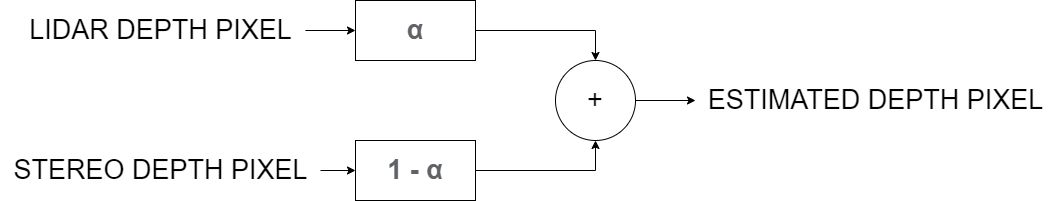
\includegraphics[width=0.9\textwidth]{CompFiltBD.jpeg}
    \caption{Complementary Filter Block Diagram}
\end{figure}

\section{TEAM WORK}

Teamwork is an essential aspect of any successful project, and this project is no exception. Our team is composed of multiple members with different backgrounds, expertise, and skills, working together to achieve a common goal. To ensure effective collaboration and communication among team members, we have chosen to use Github as our primary source control and project management platform. This allows us to easily share code, track changes, and collaborate on different parts of the project.

In addition to Github, we are also using MATLAB, Python, and the Robot Operating System (ROS) environment for our project. These tools provide us with the necessary functionality and flexibility to implement and test our sensor fusion algorithm. MATLAB, in particular, is useful for prototyping and simulating our algorithm, while Python and ROS provide us with the ability to implement and test our algorithm on real-world systems.

We also keep a logbook during the project which contains our daily progress, issues encountered, and solutions implemented. This logbook acts as a reference for team members and helps keep track of the project's history and progress. Keeping a logbook is a best practice in project management, as it helps to stay organized, keep track of progress, and document any issues that may arise.

Other papers in the field also highlighted the importance of team work, communication, and collaboration in the development of sensor fusion algorithms. For example, in their paper on sensor fusion for mobile robots, authors underline that the development of a sensor fusion algorithm is a complex task that requires a multidisciplinary team with expertise in various fields such as robotics, control systems, and computer vision. They also point out that effective communication and collaboration among team members is crucial to the success of the project.

According to \cite{daniilidis2001sensor}, sensor fusion is a complex task that has been extensively studied and is widely used in various applications. In \cite{durrant2006simultaneous}, it was stated that simultaneous localization and mapping (SLAM) is an important problem in the field of robotics that requires the integration of sensor data through sensor fusion. Additionally, in \cite{silva2020edge} the authors proposed to use edge preservation methods to increase the performance of depth map filtering for stereo vision, which can be useful for our sensor fusion algorithm.

In conclusion, effective teamwork is crucial to the success of this project, and we are utilizing a variety of tools and best practices to ensure that our team can work together effectively. Our use of Github, MATLAB, Python, and the ROS environment, as well as our logbook and regular team meetings, will help us to stay organized and work effectively together to achieve our goals.

\section{COMMENTS AND CONCLUSIONS}

In conclusion, sensor fusion is an essential component of modern technology that is used to sense and augment the environment. Our proposed project aims to develop a sensor fusion algorithm for extracting depth information using data from living organisms, specifically studying the way in which zebra fish process sensor data to produce depth information. We plan to use a legged robot for the system and cloud computing for high computing power requirements. The preliminary design of the project includes using the ZED stereo camera and Velodyne 3D LiDAR as sensors and implementing a complementary filter algorithm to fuse the depth information from the two sensors, with edge preservation methods being used as an aid to the main algorithm to increase performance.

Effective teamwork and collaboration among team members are crucial to the success of this project, and we are utilizing a variety of tools and best practices such as Github, MATLAB, Python, the Robot Operating System (ROS) environment, and a logbook to ensure that our team can work together effectively. We also have been studying the sensor fusion and alternative methodologies to implement it correctly to serve the main purpose of sensor fusion, that is reliable odometry data extraction.

In future work, we plan to improve the sensor fusion algorithm by incorporating data from the zebra fish, optimize the resolution and data rates, and test the algorithm on a legged robot with cloud computing. Additionally, we plan to implement the sensor fusion algorithm on an autonomous SLAM robot to demonstrate the usefulness of the depth information in real-world applications.

The preliminary design of our sensor fusion algorithm includes the use of the ZED stereo camera and Velodyne 3D LiDAR sensors as they are well-documented, have a large community, and are easier to use and access resources than the internal sensors of the legged robot. The sensor fusion algorithm chosen for the preliminary design is a complementary filter, which is a simple and low-performance algorithm, but it can be improved by using edge preservation methods to increase the sensor fusion performance. We have also considered the different properties, advantages, and disadvantages of the sensors to optimize the sensor fusion algorithm. The stereo vision camera and 3D lidar have different viewing angles, data formats, and sample rates, thus we have to match them by reducing the viewing angle of the 3D lidar, upsampling the lidar data, converting it to cartesian form, and using dynamic Papoulis-Gerchberg algorithm to augment the lidar data. We also aim to optimize resolution and data rates in the future work to increase the quality of the point clouds and reduce the computational effort.

In addition to the previous conclusions, it is worth noting that the preliminary design of our sensor fusion algorithm was realized using the MATLAB programming environment. This choice was made because of the wide range of tools and functions available in MATLAB for image processing and sensor data manipulation, as well as its user-friendly interface and compatibility with other programming languages such as Python and C++.

By using MATLAB, we were able to effectively implement the sensor fusion algorithm, including the complementary filter, edge preservation methods, and dynamic Papoulis-Gerchberg algorithm. We also were able to test the algorithm with sample data and evaluate its performance.

It is important to note that while the preliminary design has been realized in MATLAB, we plan to implement the final version of the sensor fusion algorithm in an appropriate programming environment for the legged robot, such as ROS, to ensure the compatibility and efficiency of the algorithm in the real-world application.

\addcontentsline{toc}{section}{REFERENCES}
\bibliographystyle{plain}
\bibliography{refs}
\end{document}